\section{Durchführung}
\label{sec:Durchführung}
Für den Versuch wird ein Drillachse wie in Abbildung \ref{fig:Drillachse} verwendet.
\begin{figure}
  \centering
  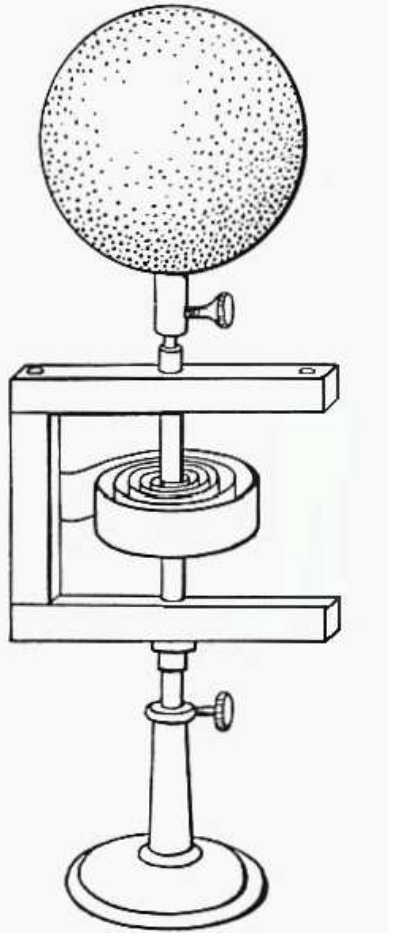
\includegraphics[width=0.14\textwidth]{Drillachse.png}
  \caption{Abbildung der Messapparatur \cite{sample}.}
  \label{fig:Drillachse}
\end{figure}
Die Apparaturkonstanten die Winkelrichtgrößen $D$ und das Trägheitsmoment $I_D$
werden bestimmt. Dafür wird an der Drillachse in einem Abstand $r$ vom Mittelpunkt
eine Federwaage eingehängt, um den Winkel $\varphi$ ausgelenkt und mit Gleichung
\eqref{eqn:Winkelrichtgroesse} die Winkelrichtgröße bestimmt.
Um das Trägheitsmoment $I_D$ zu bestimmen, wird an der Drillachse eine möglichst
masselosen Stange mit zwei Gewichten senkrecht zur Drehachse befestigt. Das System
wird in Schwingung versetzt und die Schwingungsdauer $T$ gemessen. Die Schwingungsdauern
werden quadratisch zu den Abstandsquadraten aufgetragen, dann wird das Eigenträgheitsmoment
$I_D$ mittels linearer Regression und Gleichung \eqref{eqn:Periodetorrosion} bestimmt.
Als nächstes werden die Trägheitsmomente von zwei verschiedenen Körpern durch die
Gleichung \eqref{eqn:Periodetorrosion} bestimmt werden. Dafür werden die Körper
auf der Drillachse befestigt, das System in Schwingung versetzt und die Schwingungsdauer
von fünf Perioden gemessen.
Nun wird nach der selben Methode das Trägheitsmoment einer Puppe in zwei verschiedenen
Haltungen gemessen. Um die Ergebnisse zu vergleichen werden die Formen der Körper
und Puppen vermessen und ihr Gewicht bestimmt. Bei der Puppe werden dafür die Körperteile
Kopf, Beine, Arme und Rumpf als Zylinder genähert.
